\section{Multilevel Monte Carlo Methoden}

\begin{frame}[c]
	\frametitle{Idee der Multilevel Monte Carlo Methode}
	\textbf{Ziel:} Gleichbleibende Genauigkeit bei geringerem Rechenaufwand.
	\newline
	\newline
	\underline{Im Allgemeinen:}
	\newline
	\noindent\hspace*{5mm}Gegeben: Wahrscheinlichkeitsraum $(\Omega,\mathcal{A},\mathbb{P})$, \newline
	\noindent\hspace*{21mm}(reelle) Zufallsvariable $P$
	\newline
	\noindent\hspace*{5mm}Gesucht: $\mathbb{E}[P]$
	\newline
	\newline
	\onslide<2->{\textbf{Ansatz:} Approximieren $P$ durch eine Folge $\{P_l\}_{l\in\mathbb{N}}$ für die gilt:
	\begin{tabular}[h]{p{0.01\linewidth}p{0.87\linewidth}}
		\textcolor{green}{$\boldsymbol{\oplus}$} & Approximationsfehler von $P_l$ sinkt mit wachsendem $l$.\\
		\textcolor{red}{$\boldsymbol{\ominus}$} & Rechenaufwand für Simulationen steigt mit wachsendem $l$ monoton.
	\end{tabular}
	}
	\newline
	\newline
	\onslide<3->{\textbf{Idee:} Vorteile von kleinen und großen Leveln $l$ kombinieren, um $\mathbb{E}[P_L]$ für ein $L$ als Näherung an $\mathbb{E}[P]$ zu berechnen.}
\end{frame}

%\begin{frame}[c]
%	\frametitle{Beispiel: Kurssimulationen}
%	Unterschiedliche Diskretisierungsweiten in unterschiedlichen Leveln ($M=2^l$ Simulationspunkte in Level $l$):
%	\begin{center}
%		\begin{figure}
%			\centering
%			\subfloat[$M=4$ \label{pic:asset_prices_2}]{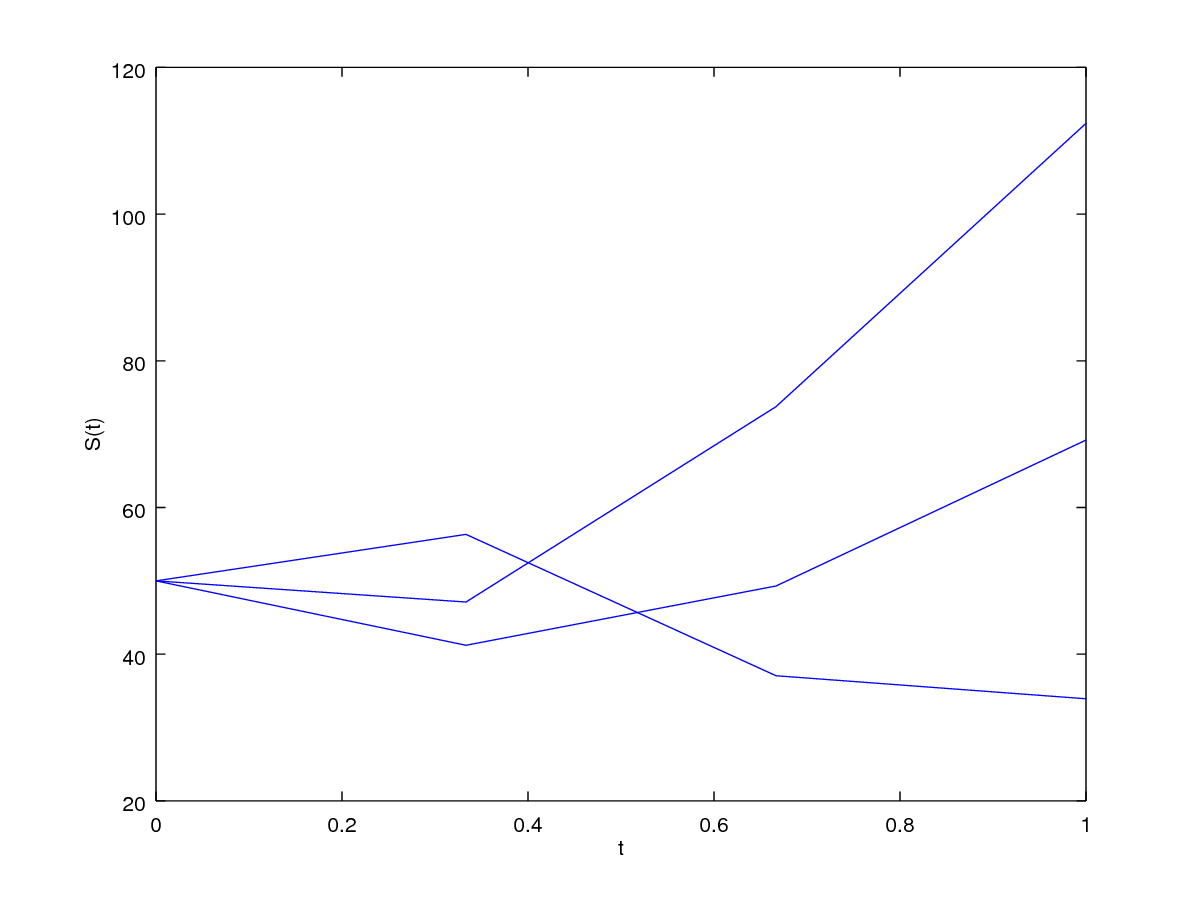
\includegraphics[width=0.45\linewidth]{figures/asset_prices_2.png}}
%			\hfill % alternativ auch \hspace{1cm} für genaue Angaben
%			\subfloat[$M=8$ \label{pic:asset_prices_3}]{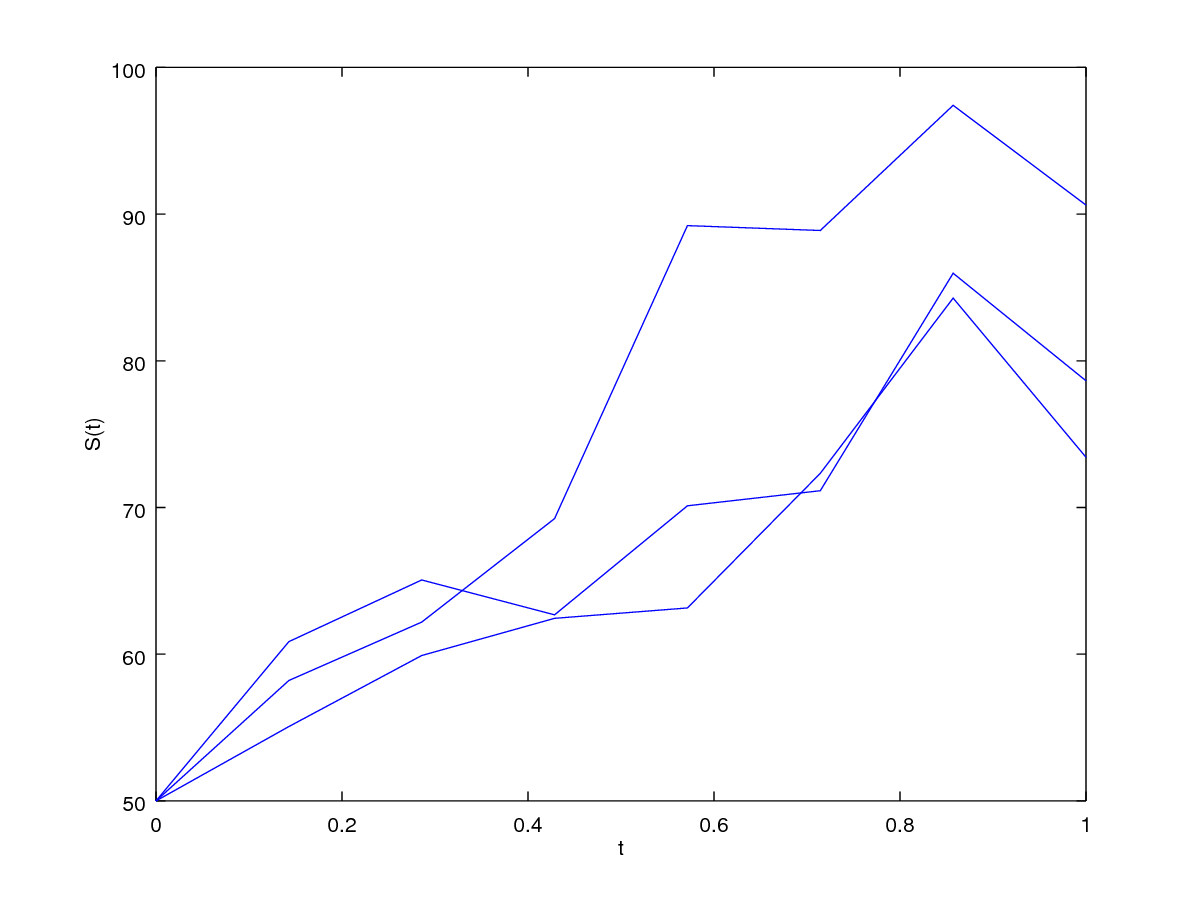
\includegraphics[width=0.45\linewidth]{figures/asset_prices_3.png}}
%		\end{figure}
%	\end{center}
%\end{frame}
%
%\begin{frame}[c]
%	\frametitle{Beispiel: Kurssimulationen}
%	Unterschiedliche Diskretisierungsweiten in unterschiedlichen Leveln ($M=2^l$ Simulationspunkte in Level $l$):
%	\begin{center}
%		\begin{figure}
%			\centering
%			\subfloat[$M=16$ \label{pic:asset_prices_4}]{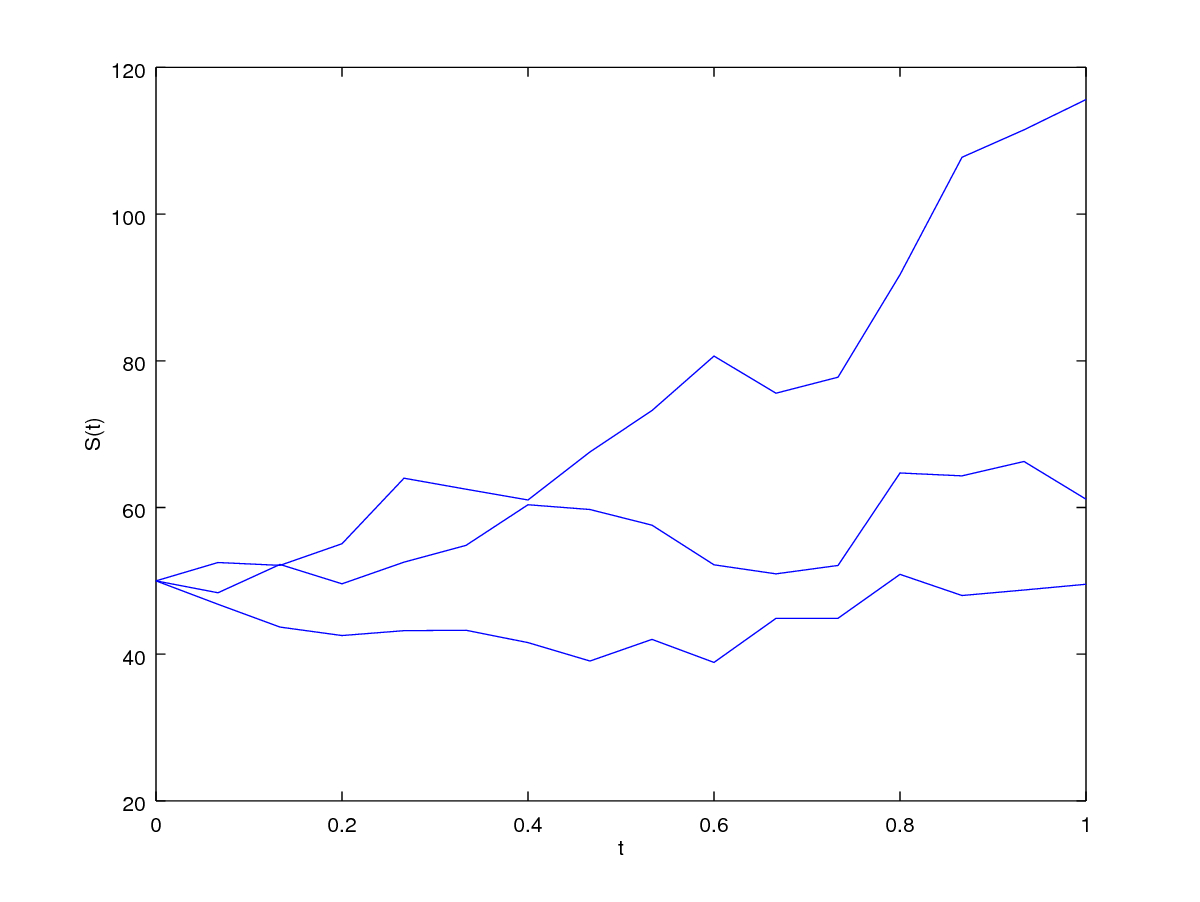
\includegraphics[width=0.45\linewidth]{figures/asset_prices_4.png}}
%			\hfill % alternativ auch \hspace{1cm} für genaue Angaben
%			\subfloat[$M=32$ \label{pic:asset_prices_5}]{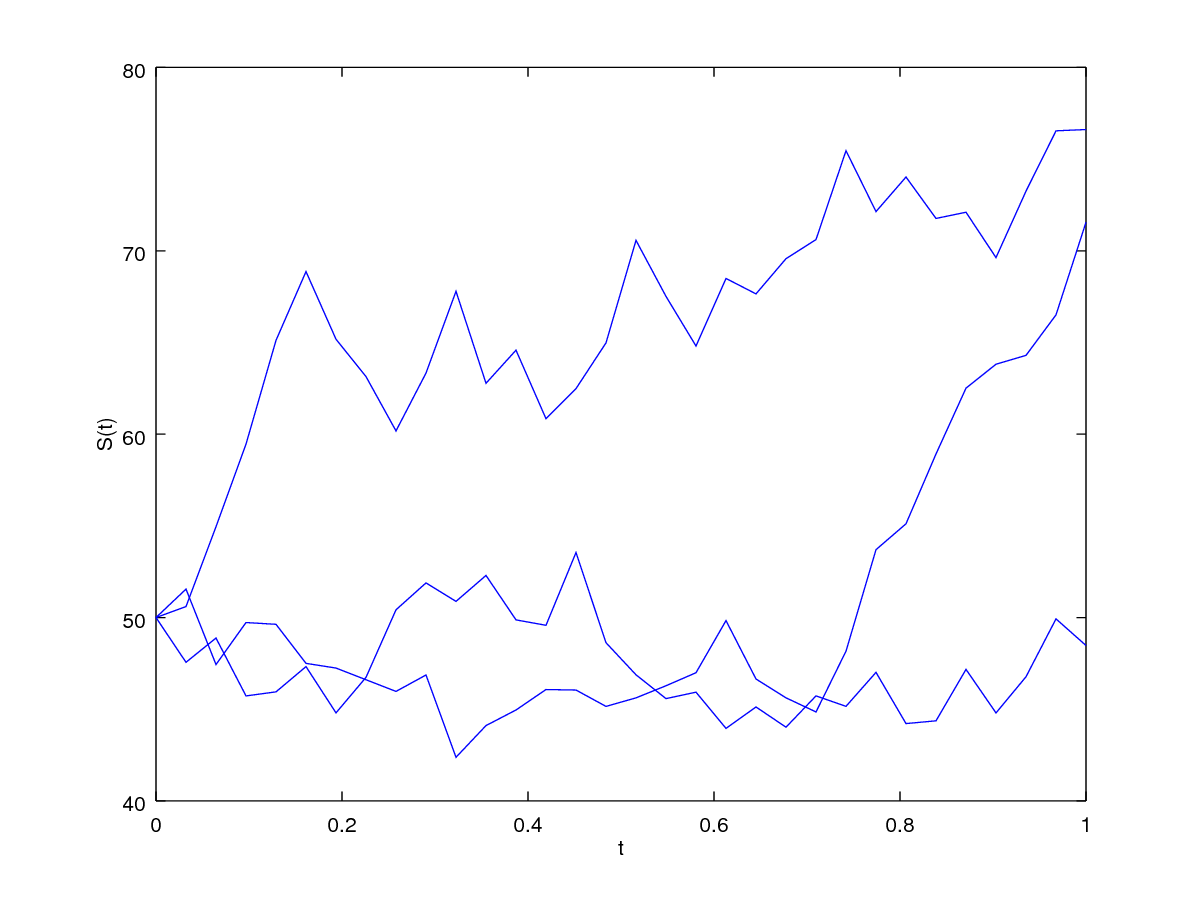
\includegraphics[width=0.45\linewidth]{figures/asset_prices_5.png}}
%		\end{figure}
%	\end{center}
%\end{frame}

\begin{frame}[c]
	\frametitle{Idee der Multilevel Monte Carlo Methode}
	Wir nutzen folgende Teleskopsumme:
	\begin{align}
		\mathbb{E}[P_L]=\mathbb{E}[P_0]+\sum\limits_{l=1}^L \mathbb{E}[P_l-P_{l-1}]. \label{teleskopsummeMultilevelMonteCarloKurssimulation}
	\end{align}
	\onslide<2->{Einsetzen eines Schätzers wie in Formel \eqref{simpleMonteCarloKurssimulation} für jeden Erwartungswert ergibt den Schätzer $Y$,
	\begin{align}
		Y:=\frac{1}{N_0}\sum\limits_{i=1}^{N_0}P_0^{(0,i)}+\sum\limits_{l=1}^L\left(\frac{1}{N_l}\sum\limits_{i=1}^{N_l}P_l^{(l,i)}-P_{l-1}^{(l,i)}\right), \label{teleskopsummeMultilevelMonteCarloKurssimulationMitSchaetzer}
	\end{align}
	für $\mathbb{E}[P_L]\approx\mathbb{E}[P]$.
	}
\end{frame}

\begin{frame}
	\frametitle{Fehler der Multilevel Monte Carlo Methode}
	Es gilt 
	\[
		\mathbb{E}[Y]=\mathbb{E}[P_L]
	\]
	und
	\[
		\mathbb{V}[Y]=\sum\limits_{l=0}^{L}\frac{1}{N_l}\mathbb{V}[P_l-P_{l-1}]
	\]
	wobei $P_{-1}\equiv 0$ gesetzt wird.
	\newline
	\onslide<2->{Dies ergibt einen mean squared error ($MSE$) von
	\begin{eqnarray}
		MSE&=&\mathbb{E}\left[(Y-\mathbb{E}[P])^2\right]\notag\\
		&=&\mathbb{V}[Y]+(\mathbb{E}[Y]-\mathbb{E}[P])^2\notag\\
		&=&\underbrace{\sum\limits_{l=0}^{L}\frac{1}{N_l}\mathbb{V}[P_l-P_{l-1}]}_{\substack{\text{Stichproben-Fehler}}}\ +\underbrace{(\mathbb{E}[P_L-P])^2}_{\substack{\text{Approximationsfehler}}}. \label{MSEMultilevelMonteCarlo}
	\end{eqnarray}}
\end{frame}

\begin{frame}[c]
	\frametitle{Konkreter: Zwei-Level Monte Carlo Methode}
	Zwei-Level Schätzer:
	\[
	Y:=\frac{1}{N_0}\sum\limits_{i=1}^{N_0}P_0^{(0,i)}+\frac{1}{N_1}\sum\limits_{i=1}^{N_1}\underbrace{P_1^{(1,i)}-P_0^{(1,i)}}_{\substack{\text{Differenz von }P_1\text{ und }P_0\\ \text{bei gleichen Samples}}}
	\]
	\newline
	\newline
	\onslide<2->{\textbf{Fragen:}
	\begin{itemize}
		\item Wie verhalten sich Berechnungskosten und Varianz des Schätzers?
		\newline
		\item Wie sollten $N_0$ und $N_1$ am besten gewählt werden?
	\end{itemize}}
\end{frame}

\begin{frame}[c]
	\frametitle{Berechnungskosten und Varianz des Zwei-Level-Schätzers}
	Seien $C_0$ und $C_1$ die Berechnungskosten für ein Sample von $P_0$ und $P_1-P_0$.
	\newline
	\underline{Gesamtkosten:} $C=N_0 C_0+N_1 C_1$
	\newline
	\newline
	\onslide<2->{Seien $V_0$ und $V_1$ die Varianzen von $P_0$ und $P_1-P_0$.
	\newline
	\underline{Varianz des Schätzers:} $V=\frac{V_0}{N_0}+\frac{V_1}{N_1}$}
	\newline
	\newline
	\onslide<3->{Sei $C$ fest. Wir minimieren $V$, wobei $N_0,N_1$ reelle Variablen seien.
	\newline
	\newline
	$\Rightarrow$ \textbf{Lagrange-Multiplikatoren-Methode}}
\end{frame}

\begin{frame}[c]
	\frametitle{Lagrange-Multiplikatoren-Methode}
	Lagrange-Funktion:
	\[
		\mathcal{L}((N_0,N_1),\mu)=\frac{V_0}{N_0}+\frac{V_1}{N_1}+\mu\cdot(N_0 C_0+N_1 C_1-C)
	\]
	\newline
	\onslide<2->{Karush-Kuhn-Tucker-Bedingungen:
	\begin{eqnarray}
	&&0\stackrel{!}{=}\nabla_{(N_0,N_1)}\mathcal{L}=\begin{bmatrix}
		-V_0/N_0^2+\mu C_0\\-V_1/N_1^2+\mu C_1
		\end{bmatrix} \notag \\
	&\Leftrightarrow&N_0=\sqrt{\frac{V_0}{\mu C_0}}\ \ \wedge\ \ N_1=\sqrt{\frac{V_1}{\mu C_1}}\label{N0N1Lagrange}
	\end{eqnarray}}
\end{frame}

\begin{frame}[c]
	\frametitle{Varianz}
	\textbf{Ziel:} Gesamtvarianz $V=\epsilon^2/2$
	\newline
	\newline
	Mit Gleichung \eqref{N0N1Lagrange} folgt:
	\begin{eqnarray}
		&&\epsilon^2/2=V\notag\\
		&\Leftrightarrow&\epsilon^2/2=V_0/N_0+V_1/N_1\notag\\
		&\Leftrightarrow&\epsilon^2/2=\sqrt{\mu V_0C_0}+\sqrt{\mu V_1C_1}\notag\\
		&\Leftrightarrow&\epsilon^2/2=\sqrt{\mu}(\sqrt{V_0C_0}+\sqrt{V_1C_1})\notag\\
		&\Leftrightarrow&\sqrt{\mu}=\frac{\epsilon^2}{2(\sqrt{V_0C_0}+\sqrt{V_1C_1})} \label{sqrtMuLagrange}
	\end{eqnarray}
\end{frame}

\begin{frame}[c]
	\frametitle{Rechenaufwand}
	Mit \eqref{N0N1Lagrange} und \eqref{sqrtMuLagrange} gilt für den Rechenaufwand $C$ nun:
	\begin{eqnarray}
		C&=&N_0C_0+N_1C_1\notag\\
		&=&\sqrt{\frac{V_0}{\mu C_0}}\ C_0+\sqrt{\frac{V_1}{\mu C_1}}\ C_1\notag\\
		&=&\frac{1}{\sqrt{\mu}}(\sqrt{V_0C_0}+\sqrt{V_1C_1})\notag\\
		&=&2\ \frac{(\sqrt{V_0C_0}+\sqrt{V_1C_1})^2}{\epsilon^2}
	\end{eqnarray}
\end{frame}

\begin{frame}[c]
	\frametitle{Optimale Anzahl von Samples}
	Zusammenfassend ergibt sich:
	\[
		N_0=\frac{1}{\sqrt{\mu}}\sqrt{\frac{V_0}{C_0}}=2\left(\frac{\sqrt{V_0C_0}+\sqrt{V_1C_1}}{\epsilon^2}\right)\sqrt{\frac{V_0}{C_0}}
	\]
	\[
		N_1=\frac{1}{\sqrt{\mu}}\sqrt{\frac{V_1}{C_1}}=2\left(\frac{\sqrt{V_0C_0}+\sqrt{V_1C_1}}{\epsilon^2}\right)\sqrt{\frac{V_1}{C_1}}
	\]
	\newline
	\newline
	\newline
	$\rightsquigarrow$ Alle Resultate lassen sich analog auf $L>1$ übertragen.
\end{frame}